\documentclass{acm_proc_article-sp}
\usepackage{graphicx}

\begin{document}

\title{A Reasonably Fast and Fully Capable JVM in JavaScript}

\numberofauthors{4}
\author{
\alignauthor Michael Bebenita
\alignauthor Brendan Dahl
\and
\alignauthor Marco Castelluccio
\alignauthor Myk Melez
\and
\alignauthor Andreas Gal
}

\maketitle
\begin{abstract}
Dramatic improvements in browser performance have now made JavaScript a viable compilation target for a wide range of programming languages.
While targetting JavaScript is fairly easy, navigating optimization tiers wrapped in arcane magic and mystery make squeezing performance out of modern JavaScript engines incredibly difficult.
In this paper we explore the implementation of a fully capable Java virtual machine.
One that supports: class loading, interpretation, dynamic compilation, on-stack-replacement, deoptimization, threading, synchronization, garbage collection, finalization, many of the features that make Java, Java.
\end{abstract}

% \category{D.3.4}{Programming Languages}{Processors}

\terms{Languages, Design}

\keywords{ACM proceedings, \LaTeX, text tagging}

\section{Introduction}

Like it or not, JavaScript is the de facto lingua franca. ...
Lots of attempts at compiling to the web, C/C++ via Emscripten has be highly successful.
Java attempts have not been as successful, too slow, large code size.
Java needs class loading, it needs faster startup, low 
We believe compiling Java to JavaScript should be faster than writing JavaScript by hand.

The web pptimize for size and startup, not throughput.

\section{System Constraints}

In JavaScript you can't do this and that. No threads, no weak references, you can't do synch I/O, etc. ...
In JavaScript you have to pay for your cake before you eat it, vm code size matters.

\section{Motivation}

\section{Implementation}

\subsection{Class Loading}

Before the JVM can execute any code it must first load it.
Java classes are packaged in \texttt{.class} files and stored compressed in archive \texttt{.jar} files.
Decompressing \texttt{.jar} files is the first step in building a JVM in JavaScript and the first sign of the troubles ahead.

\subsubsection{GZip}

Archive files typically use the \texttt{DEFLATE} algorithm.
There are many JavaScript implementations of this algorithm, but none that we've been satisfied with in terms of performance.
...

\subsubsection{Class File Representation}

The most obvious way to deal with Java \texttt{.class} files is to parse them into a JavaScript friendly object graph.
This is convenient but it has several severe disadvantages:
\begin{enumerate}
\item The \texttt{.class} file structure is directly accessible and doesn't need to be parsed ahead-of-time.
Parsing introduces a significant latency delay and should be deferred as long much as possible. 
\item The \texttt{.class} file structure is compact. Reflecting this into an JavaScript object graph more than doubles the size of the data structure.
\end{enumerate}

To work around these limitations and still provide a convenient way to represent \texttt{.class} files, we create views on the underlying \texttt{.class} file buffer. Access to most properties is performed via accessor getters that lazily construct additionaly subviews as needed. The advantage of this approach is that most of the data is kept in the original buffer and never reflected into JavaScript properties.

\begin{figure}[htbp]
\begin{center}
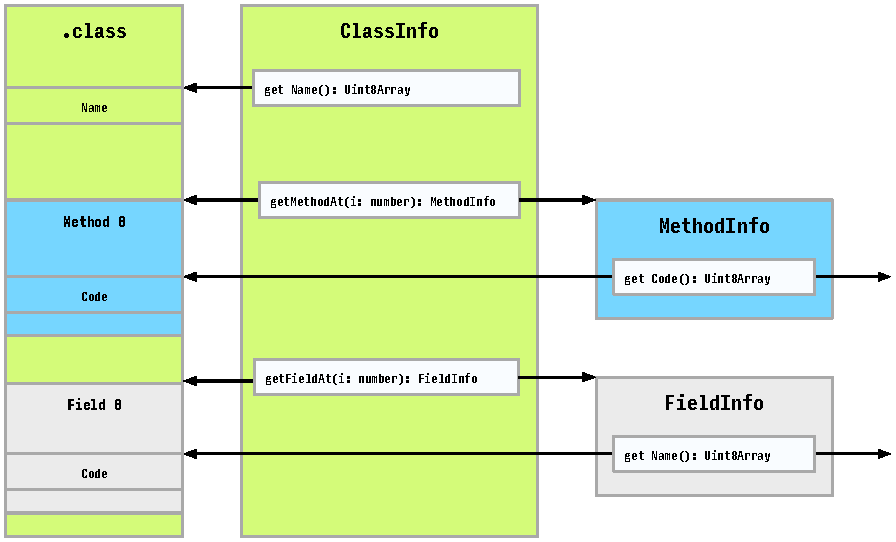
\includegraphics[width=200px]{classInfo.pdf}
\caption{ClassInfo TypedArray Views}
\label{default}
\end{center}
\end{figure}

\subsubsection{Strings}

While its tempting to reflect Java strings as JavaScript strings, it turns out that its a lot more effective to keep them in their original representation.
Strings in the JavaScript engine are heavily optimized. Taking advantage of this fact at first seems like a good idea, not only for convenience but also for performance reasons.
Unfortunately reflecting Java strings as JavaScript strings caused a lot of unintended consequences.
Decoding Java's UTF-8 encoding of strings is slow and usually unnecessary. Much of the \texttt{.class} file 


\subsection{Stack Layout}

\subsubsection{Object Arrays}

\subsubsection{Typed Arrays}

\subsection{Interpreter}

\subsubsection{Switch Loop}

\subsubsection{Hosted Interpreter}

\subsection{Interpreter}

\subsection{Just-in-Time Compiler}

\subsubsection{Relooper}

\subsection{Threading}

\subsubsection{Scheduling}

\subsubsection{Asynchronous I/O}

\subsection{Unwinding}

\subsection{On-Stack-Replacement}

\subsection{Garbage Collection}

\subsection{Performance Tuning}

\subsubsection{Startup Speed}

\subsubsection{Memory Usage}

\subsection{Host VM Tuning}

\subsection{Citations}

\subsection{Evaluation}

\section{Related Work}

\section{Conclusions}

\bibliographystyle{abbrv}
\bibliography{sigproc}  % sigproc.bib is the name of the Bibliography in this case

\end{document}
